% Copyright 2012 David W. Hogg (NYU).  All rights reserved.

\documentclass[pdftex]{beamer}
\usepackage{amssymb,amsmath,mathrsfs}
\usecolortheme{default}

%%% color commands
\newcommand{\whiteonblack}{%
  \colorlet{fg}{white}
  \colorlet{bg}{black}
  \setbeamercolor{normal_text}{fg=white,bg=black}
  \setbeamercolor{background canvas}{fg=white,bg=black}
  \setbeamercolor{alerted_text}{fg=yellow}
  \setbeamercolor{example_text}{fg=white}
  \setbeamercolor{structure}{fg=white}
  \setbeamercolor{palette_quaternary}{fg=white}
}
\newcommand{\blackonwhite}{%
  \colorlet{fg}{black}
  \colorlet{bg}{white}
  \setbeamercolor{normal_text}{fg=black,bg=white}
  \setbeamercolor{background canvas}{fg=black,bg=white}
  \setbeamercolor{alerted_text}{fg=blue}
  \setbeamercolor{example_text}{fg=black}
  \setbeamercolor{structure}{fg=black}
  \setbeamercolor{palette_quaternary}{fg=black}
}
\xdefinecolor{pink}{rgb}{1.0,0.9,0.9}

%%% size and shape commands
\newlength{\figurewidth}
\setlength{\figurewidth}{0.9\textwidth}
\newlength{\figureheight}
\setlength{\figureheight}{0.9\textheight}

%%% text commands
\newcommand{\project}[1]{\textsl{#1}}
  \newcommand{\an}{\project{Astrometry.net}}
  \newcommand{\flickr}{\project{flickr}}
  \newcommand{\gaia}{\project{Gaia}}
  \newcommand{\galex}{\project{GALEX}}
  \newcommand{\GALEX}{\galex}
  \newcommand{\hst}{\project{HST}}
  \newcommand{\hipparcos}{\project{Hipparcos}}
  \newcommand{\lsst}{\project{LSST}}
  \newcommand{\sdss}{\project{SDSS}}
  \newcommand{\sdssiii}{\project{SDSS-III}}
  \newcommand{\boss}{\sdssiii\ \project{BOSS}}
  \newcommand{\osss}{\project{OSSS}}
  \newcommand{\vo}{\project{VO}}
  \newcommand{\rttd}{\project{Right Thing To Do}$^{\mbox{\scriptsize\sffamily{TM}}}$}
\newcommand{\foreign}[1]{\textit{#1}}
\newcommand{\latin}[1]{\foreign{#1}}
  \newcommand{\cf}{\latin{cf.}}
  \newcommand{\eg}{\latin{e.g.}}
  \newcommand{\etal}{\latin{et~al.}}
  \newcommand{\etc}{\latin{etc.}}
  \newcommand{\ie}{\latin{i.e.}}
  \newcommand{\vs}{\latin{vs.}}

%%% math-mode commands
\newcommand{\unit}[1]{\mathrm{#1}}
  \newcommand{\rad}{\unit{rad}}
  \newcommand{\s}{\unit{s}}
  \newcommand{\yr}{\unit{yr}}
  \newcommand{\km}{\unit{km}}
  \newcommand{\kmps}{\km\,\s^{-1}}
\newcommand{\mmatrix}[1]{\boldsymbol{#1}}
\newcommand{\tv}[1]{\boldsymbol{#1}}
\newcommand{\dd}{\mathrm{d}}
\newcommand{\given}{\,|\,}
 % hogg standard colors

\newcommand{\fobs}{f_i}
\newcommand{\sobs}{s^2_i}
\newcommand{\ftrue}{f_i^*}

\begin{document}

\begin{frame}
  \frametitle{situation normal}
  imagine that
  \begin{itemize}
  \item you \emph{don't believe the errors} you have been given,
  \item the data are \emph{highly censored},
  \item you \emph{aren't given quantitative upper limit information}, and
  \item you \emph{don't know why the data were censored} and expect that it is a stochastic function of time
  \end{itemize}
\end{frame}

\begin{frame}
  \frametitle{\project{ASAS} data}
  \only<1>{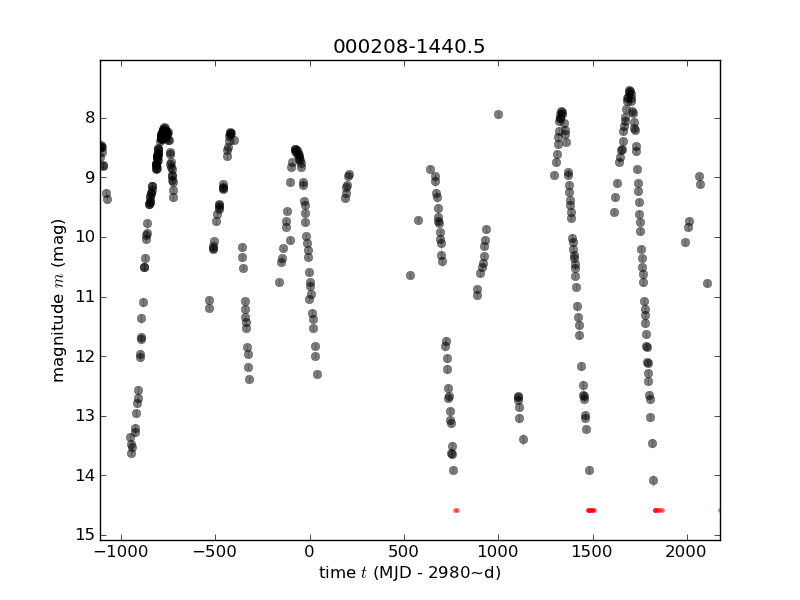
\includegraphics[width=\textwidth]{bestfit_000208-1440_5_orig.png}}
  \only<2>{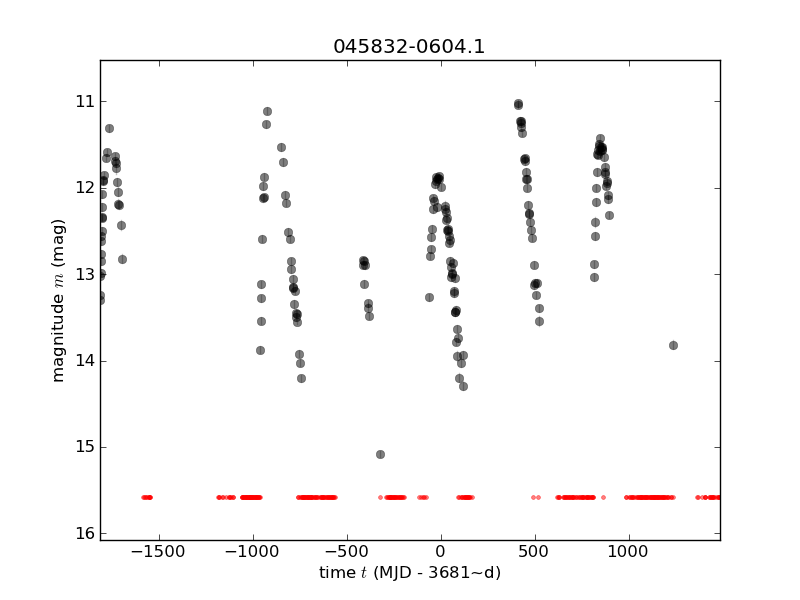
\includegraphics[width=\textwidth]{bestfit_045832-0604_1_orig.png}}
  \only<3>{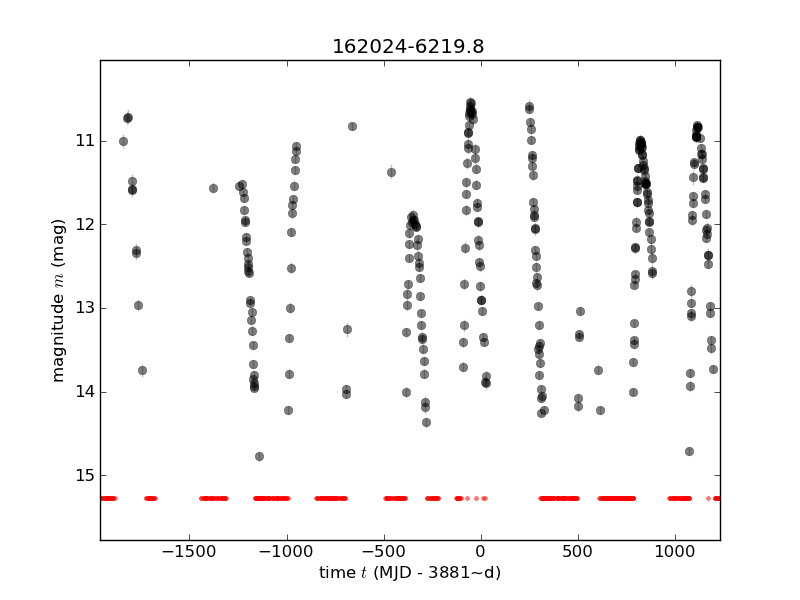
\includegraphics[width=\textwidth]{bestfit_162024-6219_8_orig.png}}
\end{frame}

\begin{frame}
  \frametitle{principal collaborators}
  \begin{itemize}
  \item Joey Richards (Berkeley Statistics \& CTDI)
  \item James Long (Berkeley Statistics \& CTDI)
  \item Dan Foreman-Mackey (NYU Physics \& CCPP)
  \item David W. Hogg (NYU Physics \& CCPP \& Max-Planck-Institut f\"ur Astronomie)
  \item Josh Bloom (Berkeley Astronomy \& CTDI)
  \end{itemize}
\end{frame}

\begin{frame}
  \frametitle{``traditional'' period-fitting}
\begin{eqnarray}\displaystyle
\mu_i' &=& A_0 + \sum_{k=1}^K A_k\, \sin (t_i \, \omega  k) + B_k\, \cos (t_i \, \omega  k)
\nonumber \\
p(D_i|\theta,I) &=& N(D_i|\mu_i,\sigma^2_i) \quad \mbox{when $i$ is detected}
\nonumber \\
p(D|\theta,I) &=& \prod_{\mbox{detected}\,i} p(D_i|\theta,I)
\nonumber
\end{eqnarray}
\end{frame}

\begin{frame}
  \frametitle{traditional period-fitting}
  \only<1>{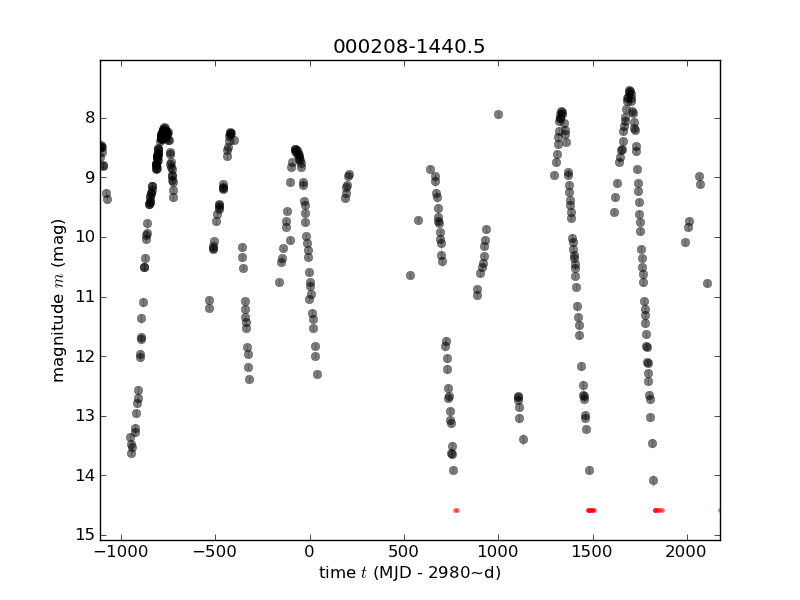
\includegraphics[width=\textwidth]{bestfit_000208-1440_5_orig.png}}
  \only<2>{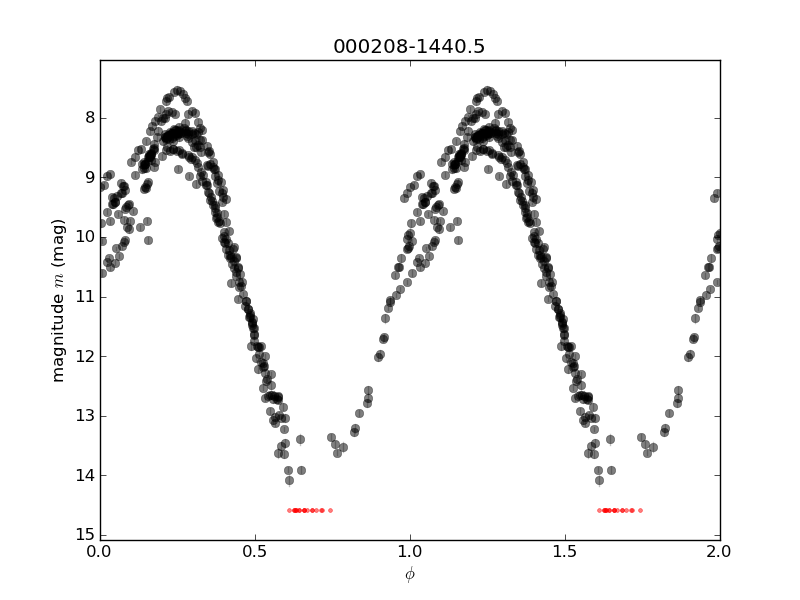
\includegraphics[width=\textwidth]{bestfit_mag_000208-1440_5_old.png}}
  \only<3>{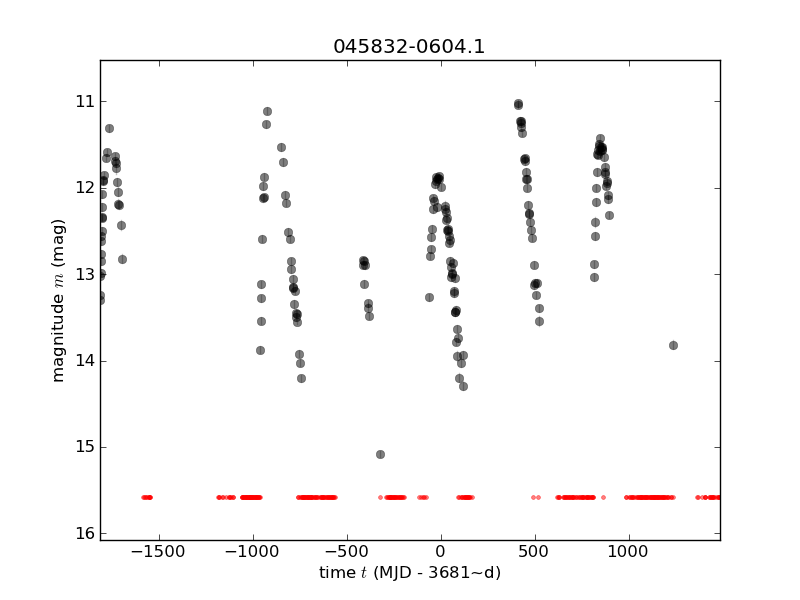
\includegraphics[width=\textwidth]{bestfit_045832-0604_1_orig.png}}
  \only<4>{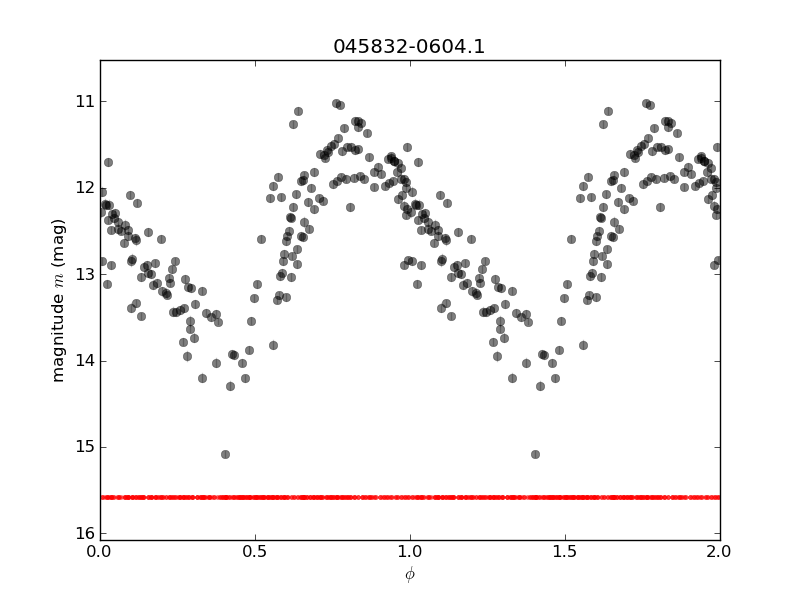
\includegraphics[width=\textwidth]{bestfit_mag_045832-0604_1_old.png}}
  \only<5>{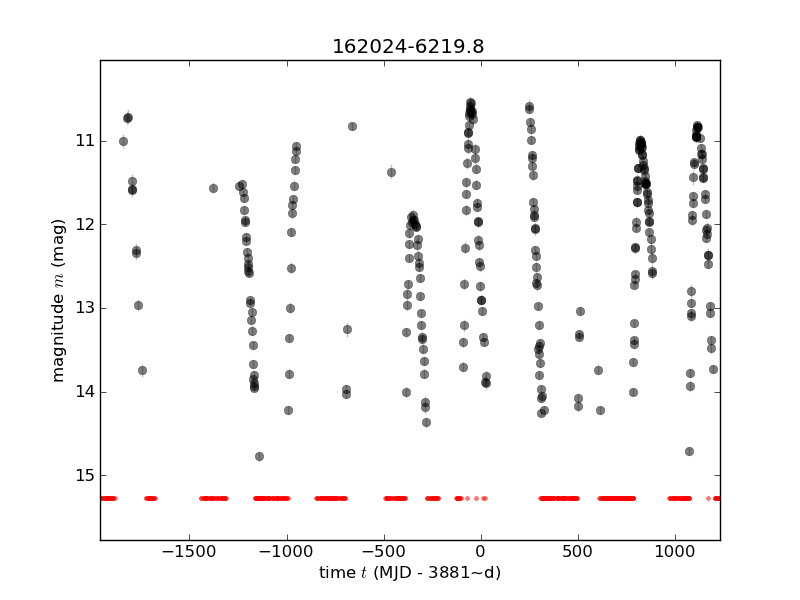
\includegraphics[width=\textwidth]{bestfit_162024-6219_8_orig.png}}
  \only<6>{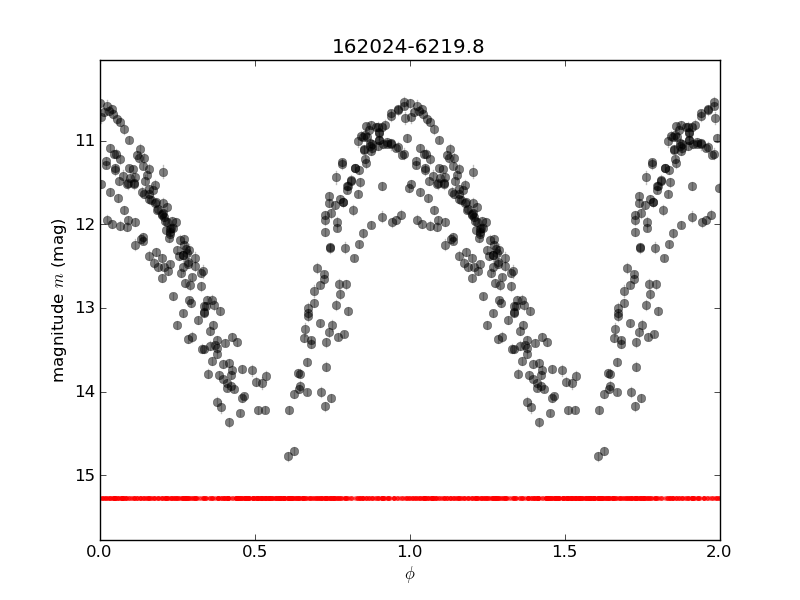
\includegraphics[width=\textwidth]{bestfit_mag_162024-6219_8_old.png}}
\end{frame}

\begin{frame}
  \frametitle{our model}
\begin{eqnarray}\displaystyle
\mu_i' &=& A_0 + \sum_{k=1}^K A_k\, \sin (t_i \, \omega  k) + B_k\, \cos (t_i \, \omega  k)
\nonumber \\
\ftrue &=& \mu_i + e_i
\nonumber \\
\fobs &=& \left\{\begin{array}{ll}
  \ftrue & \mbox{if $\ftrue \ge b_i$} \\
  \texttt{NA} & \mbox{if $\ftrue < b_i$} \\
\end{array} \right.
\nonumber \\
p(b_i|\theta) &=& N(b_i|B,V_B)
\nonumber
\end{eqnarray}
\end{frame}

\begin{frame}
  \frametitle{our model}
\begin{eqnarray}\displaystyle
\Sigma^2_i &=& \sigma^2_i + \eta^2\,\mu_i^2
\nonumber \\
p(\fobs |\sigma^2_i,\theta,I) &=& \left\{\begin{array}{ll}
  N(\fobs | \mu_i,  \Sigma^2_i)\,  \int_{-\infty}^{\fobs} p(b_i | \theta)\, \dd b_i & \mbox{if $\fobs \ne \texttt{NA}$} \\
  \int_{-\infty}^{\infty} \int_{-\infty}^{b_i} N(\ftrue | \mu_i, \Sigma^2_i)\, p(b_i | \theta)\, \dd \ftrue\, \dd b_i & \mbox{if $\fobs = \texttt{NA}$}
\end{array}\right.
\nonumber \\
p(\fobs |\sigma^2_i,\theta,I, b_i) &=& \left\{\begin{array}{ll}
  N(\fobs | \mu_i,  \Sigma^2_i)\,  I(\fobs \ge b_i) & \mbox{if $\fobs \ne \texttt{NA}$} \\
 \int_{-\infty}^{b_i} N(\ftrue | \mu_i, \Sigma^2_i)\, \dd \ftrue & \mbox{if $\fobs = \texttt{NA}$}
\end{array}\right.
\nonumber \\
p(\sobs | \fobs, \sigma^2_i, \theta,I) &=& \left\{\begin{array}{ll}
  \Gamma (\sobs | \sigma^2_i, V_{\sigma} ) & \mbox{if $\fobs \ne \texttt{NA}$} \\
 I(\sobs = \texttt{NA})& \mbox{if $\fobs = \texttt{NA}$}
\end{array}\right.
\nonumber \\
p(\sigma^2_i|\theta, I) &=& \Gamma(\sigma^2_i | S, V_S)
\nonumber \\
p(D_i|\theta,I) &=& \int_0^{\infty} p(\fobs |\sigma^2_i,\theta,I)\, p(\sobs | \fobs, \sigma^2_i,\theta,I)\, p(\sigma^2_i | \theta, I)\,\dd \sigma^2_i
\nonumber
\end{eqnarray}
\end{frame}

\begin{frame}
  \frametitle{our model}
\begin{eqnarray}\displaystyle
p(D|\theta,I) &=& \prod_i p(D_i|\theta,I)
\nonumber \\
\theta &\equiv& (\omega, A_0, \{A_k, B_k\}_{k=1}^K, \eta^2\,\mu_i^2, B, V_B, V_{\sigma}, S, V_S)
\nonumber
\end{eqnarray}
\end{frame}

\begin{frame}
  \frametitle{our model (graphical)}
  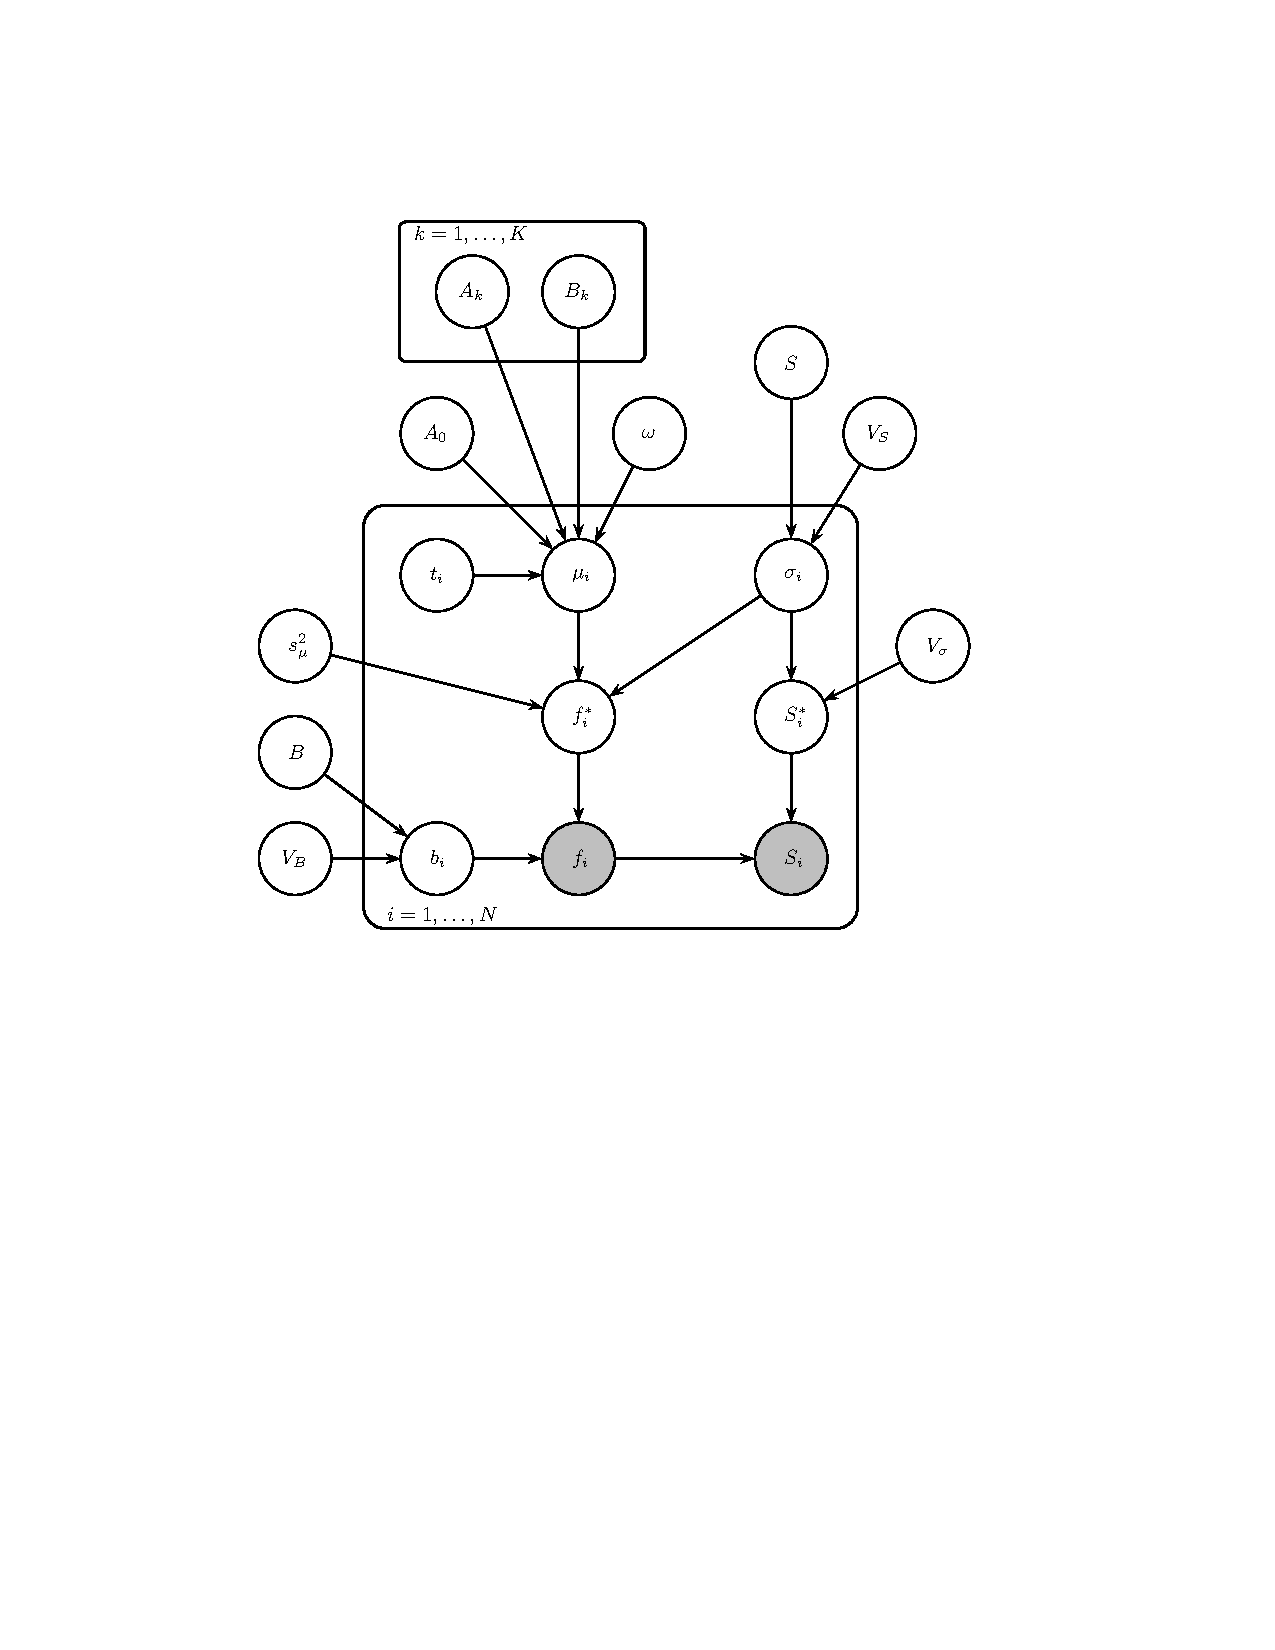
\includegraphics[trim=3cm 12cm 5cm 3cm, clip=true, width=0.85\textwidth]{../tex/gm/gm.pdf}
\end{frame}

\begin{frame}
  \frametitle{our results}
  \only<1>{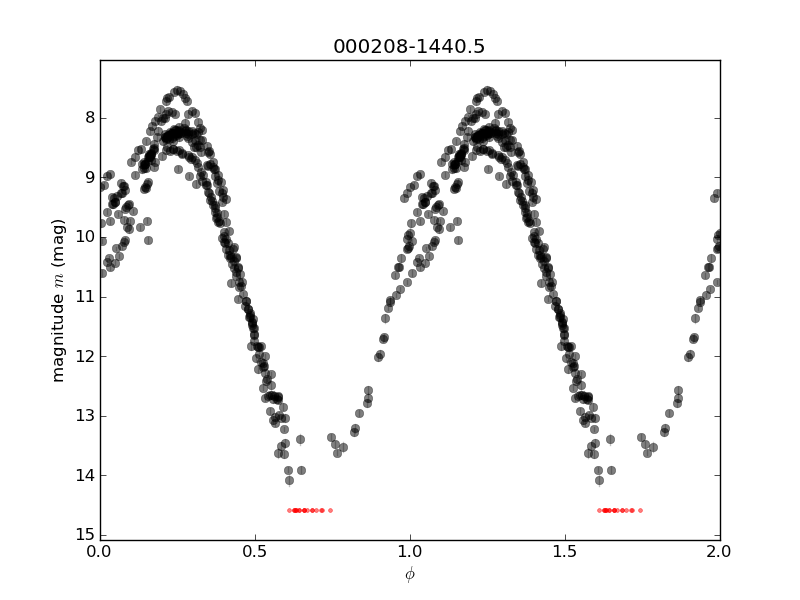
\includegraphics[width=\textwidth]{bestfit_mag_000208-1440_5_old.png}}
  \only<2>{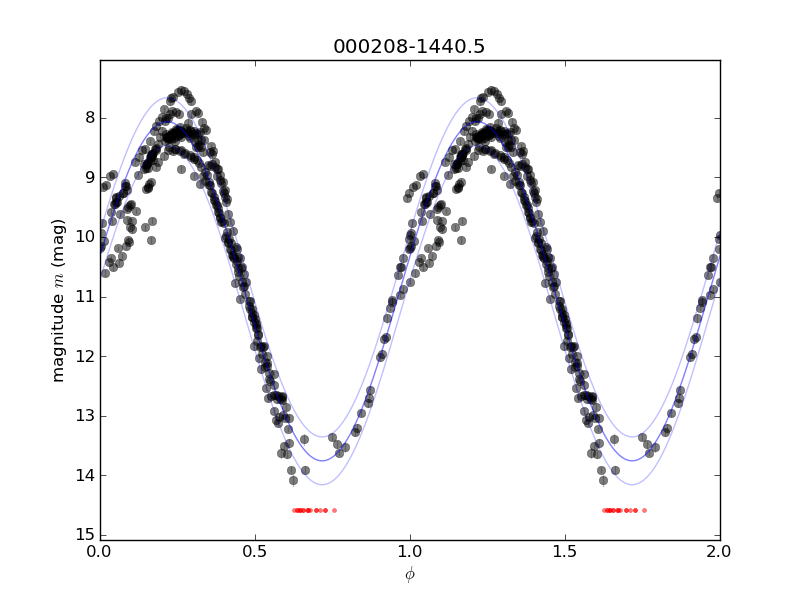
\includegraphics[width=\textwidth]{bestfit_mag_000208-1440_5_new.png}}
  \only<3>{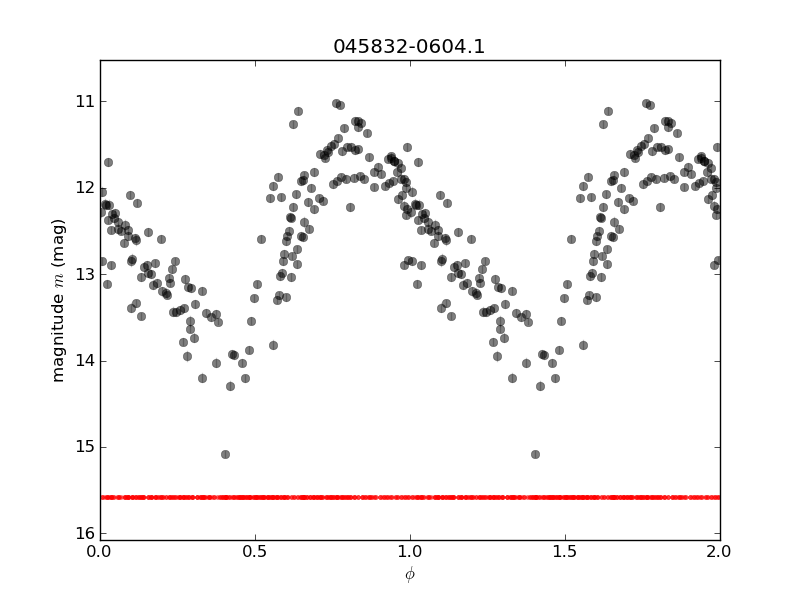
\includegraphics[width=\textwidth]{bestfit_mag_045832-0604_1_old.png}}
  \only<4>{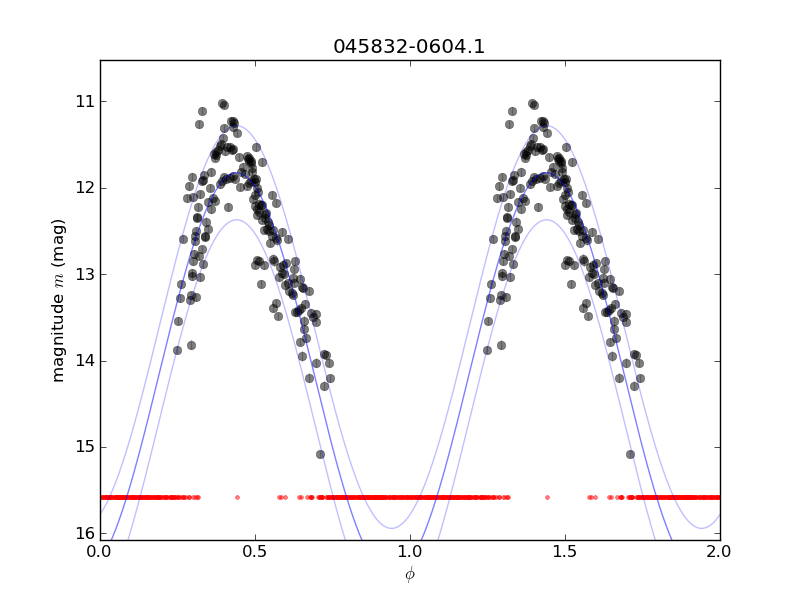
\includegraphics[width=\textwidth]{bestfit_mag_045832-0604_1_new.png}}
  \only<5>{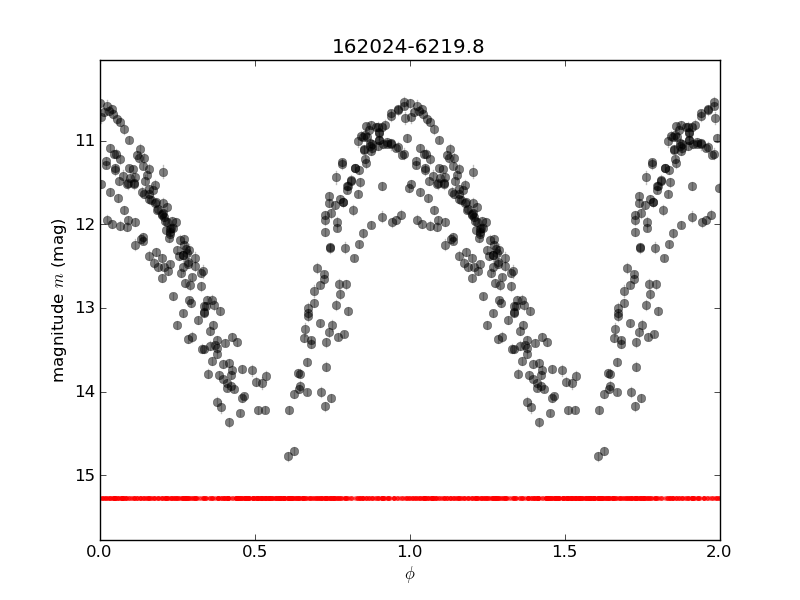
\includegraphics[width=\textwidth]{bestfit_mag_162024-6219_8_old.png}}
  \only<6>{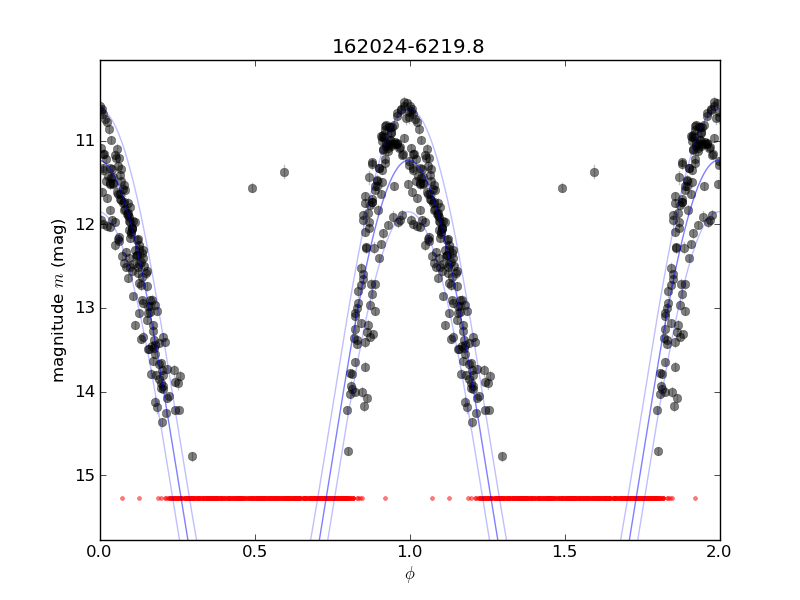
\includegraphics[width=\textwidth]{bestfit_mag_162024-6219_8_new.png}}
\end{frame}

\begin{frame}
  \frametitle{conclusions}
  \begin{itemize}
  \item even when you \emph{don't believe the errors} you have been given,
  \item even when the data are \emph{highly censored},
  \item even when you \emph{aren't given quantitative upper limit information},
  \item even when you \emph{don't know why the data were censored} and expect that it is a stochastic function of time,
  \item you \emph{can use the non-detections!}
    \begin{itemize}
    \item Key idea: The robot is insane but it isn't \emph{antagonistic}.
    \item The variations in censorship \emph{policy} are not correlated with the behavior of the source.
    \end{itemize}
  \end{itemize}
\end{frame}

\end{document}
